\h{Future Directions}

The future development of Energetically Coherent Computation requires systematic investigation across multiple domains, from molecular mechanisms to clinical applications. This section examines key research directions for validating and extending ECC's framework while maintaining rigorous scientific standards.

Several crucial areas emerge for future investigation. First, testing ECC demands sophisticated experimental approaches capable of measuring and manipulating patterns of energetic coherence while assessing their relationship to conscious experience. These methods must span multiple scales of organization, from cellular dynamics to whole-brain states, while maintaining careful control over experimental variables.

Animal models provide another essential avenue for investigation, offering natural experiments in how different neural architectures support conscious processing. The comparative study of consciousness across species helps identify which aspects of neural organization prove truly necessary for conscious experience versus those that merely represent one possible implementation.

Brain organoids and wetware computing systems present unique opportunities for studying consciousness-supporting mechanisms in controllable yet biologically authentic environments. These simplified but realistic neural tissues enable systematic investigation of how patterns of energetic coherence emerge and maintain stability, while avoiding some of the complexity and ethical challenges of working with intact brains.

Novel predictions generated by ECC provide concrete directions for empirical validation. These predictions span biological, thermodynamic, clinical, computational, and developmental domains, offering multiple avenues for testing the theory's fundamental claims. The systematic investigation of these predictions requires careful integration of multiple experimental approaches while maintaining methodological rigor.

The future directions outlined in this section suggest a comprehensive research program for advancing our understanding of consciousness through the lens of energetic coherence. Success in these endeavors requires careful balance between innovative methodological approaches and established scientific principles, while maintaining clear connection to empirically measurable phenomena.

\section{Testing ECC}

\begin{refsection}[references//0001_7_future_dirs.bib]

Testing ECC requires a multi-scale approach that examines both the physical foundations of energetic coherence and its relationship to conscious experience. The empirical validation must span multiple domains while maintaining methodological rigor.

High-temporal resolution neuroimaging combined with thermodynamic measurements offers one crucial direction for testing ECC's core predictions. Temperature mapping during neural recording can track patterns of energy flow and coherence across brain regions \cite{Watts2018}. By examining how thermal gradients correlate with conscious processing, researchers can evaluate whether energetic coherence follows the proposed constraints of neural light cones.

The analysis of scale-free brain activity provides another essential avenue for investigating ECC's framework. Recent work has demonstrated how neural dynamics maintain coherent patterns across multiple temporal and spatial scales \cite{He2014}. This scale-free organization aligns with ECC's emphasis on coordinated energy flows spanning different levels of neural architecture.

Transcriptomic analysis represents a particularly promising direction for testing ECC's predictions about regional specialization. Single-cell RNA sequencing enables detailed examination of how gene expression patterns shape local "alphabets" for conscious encoding \cite{Gallegos2020}. This molecular profiling can reveal whether regions supporting conscious processing demonstrate predicted patterns of transcriptomic diversity and energy management.

Clinical applications offer natural experiments for testing ECC's framework. Analysis of resting state networks in disorders of consciousness could reveal how different patterns of energetic disruption correlate with specific impairments \cite{Fox2010}. The relationship between network connectivity and conscious awareness may illuminate fundamental principles about how coherent energy states support conscious experience.

The investigation of brain metabolism through advanced imaging techniques enables direct testing of ECC's energetic predictions \cite{Magistretti2018}. By examining how different brain regions manage energy distribution during conscious tasks, researchers can evaluate whether conscious processing demonstrates the predicted patterns of metabolic efficiency and coherence.

Brain network analysis provides crucial tools for examining how patterns of energetic coherence emerge and maintain stability \cite{DePasquale2020}. The dynamic reorganization of neural networks during development and pathological conditions offers important opportunities for testing ECC's predictions about the relationship between network architecture and conscious processing.

These empirical approaches must be integrated within a broader theoretical framework that bridges physical mechanisms and conscious experience \cite{Northoff2020}. The systematic investigation of ECC's predictions requires careful attention to both methodological rigor and theoretical grounding to establish clear relationships between energetic coherence and conscious states.

Development of new analytical tools will prove essential for quantifying and characterizing patterns of energetic coherence. Advanced signal processing techniques combined with machine learning approaches can help identify organizational principles that might not be apparent through traditional analysis methods \cite{Buzsaki2019}. These tools must maintain careful balance between sophisticated measurement approaches and scientific validity.

The empirical validation of ECC's predictions requires sophisticated methodological frameworks that track energetic coherence across different scales of biological organization. Brain networks demonstrate remarkable plasticity during both normal development and pathological conditions \cite{Vertes2015}, providing crucial opportunities to examine how patterns of energetic coherence emerge and stabilize.

The measurement of cellular energy metabolism offers particularly valuable insights for testing ECC's framework. Advanced protocols for quantifying energy dynamics in living neural systems can reveal how different cell populations contribute to coherent energy states \cite{Zhang2019}. These measurements must track both local metabolic processes and broader patterns of energy distribution across neural tissues.

Consciousness research must bridge theoretical frameworks with empirical investigation \cite{Tononi2015}. ECC's predictions about the relationship between energetic coherence and conscious experience require careful validation through multiple complementary approaches. The integration of phenomenological reports with objective measurements presents significant methodological challenges that demand sophisticated experimental designs.

The thermodynamic properties of neural systems take on particular significance when examining consciousness through ECC's framework \cite{Sherrington2018}. Careful analysis of how brain regions manage energy flows during conscious processing can reveal whether the predicted patterns of thermodynamic efficiency emerge. This requires precise measurement of both energy consumption and information processing capabilities across different neural populations.

The temporal dynamics of conscious processing provide another crucial domain for testing ECC's predictions. Recent work has demonstrated how neural oscillations support temporal predictions and sensorimotor integration \cite{Palva2018}. The relationship between these rhythmic patterns and energetic coherence must be carefully examined to validate ECC's claims about temporal integration in conscious processing.

The neural basis of consciousness remains a central challenge in neuroscience \cite{Kucyi2017}. ECC's framework suggests specific mechanisms through which conscious experience emerges from patterns of energetic coherence. Testing these predictions requires careful integration of multiple measurement techniques while maintaining methodological rigor.

Clinical research provides unique opportunities for examining how disruptions to energetic coherence affect conscious experience. The systematic investigation of consciousness disorders can reveal whether specific patterns of coherence disruption correlate with particular impairments in conscious awareness. Longitudinal studies tracking recovery from brain injury might illuminate how consciousness re-emerges as coherent energy patterns are restored.

The development of new analytical tools for quantifying coherence represents another crucial aspect of experimental investigation. Advanced signal processing techniques for measuring phase relationships across frequencies, combined with information theoretical measures of local-to-global coherence, enable rigorous assessment of ECC's mathematical predictions. Machine learning approaches can help identify patterns in multi-scale energy dynamics that might not be apparent through traditional analysis methods.

The empirical investigation of ECC's predictions requires careful attention to how energetic coherence spans multiple scales of neural organization. The thermodynamic properties of neural information processing provide crucial constraints on how conscious systems maintain coherent states \cite{Sherrington2018}. Advanced imaging techniques must track both local energy dynamics and broader patterns of coherence across neural tissues.

Real-time metabolic mapping offers essential data about energy dynamics in conscious systems. Current protocols for measuring cellular energy metabolism can reveal how different neural populations contribute to coherent states \cite{Zhang2019}. These measurements must integrate analysis of both specific cellular processes and broader patterns of energy distribution across brain regions. 

Brain network analysis provides another vital avenue for testing ECC's predictions about conscious processing. Recent work has demonstrated how neural networks maintain complex patterns of coordination across multiple temporal scales \cite{Palva2018}. The relationship between these network dynamics and conscious experience must be carefully examined to validate ECC's claims about how coherent energy states support consciousness.

Clinical monitoring presents unique opportunities for testing ECC's framework in human subjects. The analysis of resting state networks in consciousness disorders could reveal how different patterns of energetic disruption correlate with specific impairments \cite{Fox2010}. Studies tracking coherence patterns during emergence from anesthesia or monitoring energy dynamics in disorders of consciousness may validate the theory's predictions about conscious state transitions.

The development of new analytical tools for quantifying coherence remains crucial. Brain network analysis techniques can reveal how patterns of energetic organization emerge and stabilize \cite{DePasquale2020}. Machine learning approaches may help identify organizational principles that are not apparent through traditional analysis methods \cite{Buzsaki2019}.

The neural basis of consciousness requires investigation through multiple complementary approaches \cite{Kucyi2017}. ECC's framework suggests specific mechanisms through which conscious experience emerges from patterns of energetic coherence. Testing these predictions requires careful integration of phenomenological reports with objective measurements while maintaining methodological rigor.

The success of these experimental approaches depends fundamentally on developing new technologies and methods capable of capturing the complex, dynamic nature of consciousness as proposed by ECC. This may require significant advances in neuroimaging, biosensors, and data analysis techniques. Future development of experimental protocols must maintain careful balance between sophisticated measurement approaches and rigorous scientific methodology.

\section{Experimental Approaches}

The empirical validation of ECC requires sophisticated experimental paradigms that can measure and manipulate energetic coherence while assessing its relationship to conscious experience. These approaches must span multiple scales of neural organization while maintaining methodological rigor and reproducibility.

Multi-modal neural recording represents a crucial foundation for testing ECC's predictions. Network neuroscience approaches combining EEG, MEG, and high-density microelectrode arrays enable tracking of coherent energy patterns across different spatial and temporal scales \cite{Bassett2017}. The integration of local field potential measurements with single-unit recordings provides crucial insight into how local coherence contributes to global conscious states.

Advanced metabolic mapping proves essential for understanding energy dynamics in conscious systems. Recent work has revealed precise energy budgets for neural computation across different brain regions \cite{Howarth2012}. Real-time measurements of glucose consumption and oxygen utilization, combined with monitoring of ATP dynamics, can reveal how conscious processing relates to energy management in neural tissues.

The development of new analytical tools for quantifying coherence represents another crucial aspect of experimental investigation. EEG microstates analysis provides valuable methods for studying the temporal dynamics of whole-brain neuronal networks \cite{Michel2018}. These techniques enable rigorous assessment of ECC's mathematical predictions about how local coherence patterns integrate into global conscious states.

Clinical monitoring offers unique opportunities for testing ECC's frameworks in human subjects. Studies of global resting-state fMRI activity have revealed important principles about how brain networks maintain coherent activity patterns \cite{Scholvinck2013}. These natural experiments in clinical settings offer crucial insight into how consciousness relates to patterns of energetic coherence in human brains.

The investigation of default mode network activity provides another vital avenue for understanding conscious processing \cite{Raichle2015}. By examining how different brain regions achieve and maintain coherent baseline states, researchers can evaluate ECC's predictions about the relationship between energy dynamics and conscious experience.

Advanced nanoelectronic devices for brain mapping enable unprecedented precision in measuring neural activity patterns \cite{Kuzum2014}. These tools provide essential capabilities for tracking how coherent energy states propagate through neural tissues at multiple scales. The development of such sophisticated recording technologies proves crucial for validating ECC's predictions about consciousness-supporting mechanisms.

The success of these experimental approaches depends fundamentally on developing new technologies and methods capable of capturing the complex, dynamic nature of consciousness as proposed by ECC. This may require significant advances in neuroimaging, biosensors, and data analysis techniques. Future development of experimental protocols must maintain careful balance between sophisticated measurement approaches and rigorous scientific methodology.

The relationship between synaptic plasticity and conscious processing provides another crucial domain for investigation. Recent work has revealed complex interactions between Hebbian plasticity and homeostatic mechanisms in neural circuits \cite{Turrigiano2017}. Understanding how these processes contribute to maintaining coherent energy states may illuminate fundamental principles about conscious processing.

These experimental considerations naturally lead us to examine how brain organoids might serve as simplified but biologically realistic systems for testing ECC's principles. The controlled nature of organoid systems, combined with their biological authenticity, offers unique opportunities for investigating how patterns of energetic coherence emerge and maintain conscious-like processing.

The experimental investigation of energetic coherence in living neural systems demands innovative technical solutions. The careful study of memory circuits through both theoretical models and empirical approaches provides crucial insights into how neural systems maintain coherent states \cite{Lisman2018}. These investigations must track both local circuit dynamics and broader patterns of network organization.

Astrocytic regulation of neural activity represents another essential domain for experimental investigation. Recent work has revealed sophisticated mechanisms through which astrocytes modulate cortical states \cite{Poskanzer2016}. Understanding how these glial cells contribute to maintaining coherent energy patterns proves crucial for validating ECC's predictions about consciousness-supporting mechanisms.

The study of calcium-independent signaling pathways offers particular insight into neural excitability regulation. Research has demonstrated how astrocytic lipid release can modulate neuronal activity through mechanisms distinct from traditional calcium signaling \cite{Chow2020}. These findings suggest multiple parallel pathways through which neural systems might maintain coherent energy states.

Energy budgets in neural computation take on special significance when examining consciousness through ECC's framework. Detailed analysis of energy consumption across different brain regions reveals remarkable efficiency in neural information processing \cite{Bezaires2013}. These energetic constraints must be carefully considered when evaluating how conscious systems maintain coherent states.

The relationship between sleep-wake cycles and brain energetics provides another crucial avenue for investigation. Recent work has illuminated how neural energy utilization varies across different behavioral states \cite{DiNuzzo2017}. Understanding these state-dependent changes in energy dynamics may reveal fundamental principles about how consciousness emerges from coherent energy patterns.

Optogenetic approaches enable precise manipulation of neural circuits during experimental investigation \cite{Yizhar2011}. These tools allow researchers to perturb specific aspects of neural processing while monitoring effects on coherent energy states. Such targeted interventions prove essential for establishing causal relationships between neural activity patterns and conscious processing.

The experimental investigation of consciousness demands careful integration of multiple measurement approaches. Theoretical frameworks for conscious processing must be grounded in empirical observations that span multiple scales of neural organization \cite{Dehaene2011}. This integration of theory and experiment remains crucial for advancing our understanding of how consciousness emerges from coherent energy dynamics.

The integration of multiple experimental approaches requires sophisticated analytical frameworks. Brain network analysis has revealed fundamental principles about how neural systems maintain coordinated activity across different scales \cite{Bassett2017}. These network approaches must be combined with detailed energy measurements to understand how conscious processing emerges from coherent states.

The relationship between neural energy consumption and information processing provides crucial insight into consciousness-supporting mechanisms. Careful analysis of energy budgets across different brain regions has revealed remarkable efficiency in neural computation \cite{Howarth2012}. Understanding these energetic constraints proves essential for validating ECC's predictions about how conscious systems maintain coherent states.

The investigation of resting-state networks offers particular value for understanding baseline consciousness. Global patterns of neural activity during rest reveal important principles about how brain networks maintain coherent states \cite{Scholvinck2013}. These intrinsic activity patterns may reflect fundamental mechanisms through which consciousness emerges from energetic coherence.

Experimental protocols must carefully balance the need for precise measurement with maintenance of natural neural dynamics. Advanced nanoelectronic devices enable unprecedented resolution in neural recording \cite{Kuzum2014}, while optogenetic techniques allow targeted manipulation of specific circuit elements \cite{Yizhar2011}. The integration of these approaches provides powerful tools for investigating how conscious processing emerges from coherent energy states.

The role of sleep in consciousness presents unique opportunities for experimental investigation. Recent work has revealed sophisticated relationships between brain energetics and sleep-wake cycles \cite{DiNuzzo2017}. Understanding how conscious states transform during sleep while maintaining the capacity for rapid awakening may illuminate fundamental principles about consciousness-supporting mechanisms.

These experimental considerations suggest multiple complementary approaches for testing ECC's predictions. By combining detailed analysis of neural energy dynamics with careful assessment of conscious states, researchers can evaluate whether patterns of energetic coherence indeed correlate with and support conscious processing as the theory predicts.

The success of this experimental program depends critically on maintaining rigorous standards while embracing innovative methodological approaches. Through careful integration of multiple measurement techniques and sophisticated analytical tools, researchers can build a comprehensive understanding of how consciousness emerges from coherent energy dynamics in biological systems.

\section{Animal Models}

The use of animal models provides crucial opportunities for testing ECC's predictions about the relationship between energetic coherence and conscious experience. Different species, with their varied neural architectures and behavioral repertoires, offer unique windows into how patterns of energetic organization support different forms of conscious processing \cite{Boly2013}.

Avian models present particularly illuminating cases for investigating ECC's framework. Despite lacking a layered neocortex, birds demonstrate sophisticated cognitive capabilities that challenge traditional assumptions about consciousness \cite{Gunturkun2016}. Their distinct neural architecture, organized through nuclear clusters rather than cortical layers, provides valuable insight into how different physical implementations can support conscious processing \cite{Clayton2015}.

The evolution of brain structure across species reveals important principles about consciousness-supporting architecture. Mosaic evolution of brain regions suggests that different aspects of conscious processing may have evolved independently in various lineages \cite{Barton2000}. This evolutionary perspective helps validate ECC's predictions about the physical requirements for consciousness while revealing multiple possible implementations.

Cephalopods offer another valuable model system due to their distributed neural architecture and sophisticated cognitive capabilities. Studies have demonstrated remarkable problem-solving abilities and potentially conscious-like behaviors in octopuses \cite{Mather2008}, despite their radically different neural organization from vertebrates. Their capacity for complex learning and memory, supported by unique neural architectures, provides crucial tests of ECC's predictions about consciousness-supporting mechanisms \cite{Teyke1989}.

Social insects present intriguing possibilities for studying emergent consciousness through collective dynamics. The sophisticated cognitive architecture of honeybee minds demonstrates how relatively simple neural systems can achieve complex information processing \cite{Menzel2001}. Their navigation capabilities and social behaviors suggest consciousness-like properties may emerge from specific patterns of neural organization even in miniaturized brains \cite{Webb2016}.

The evolutionary trajectory of centralized nervous systems provides essential context for understanding consciousness \cite{Northcutt2012}. Different organizational principles have emerged across various lineages, offering natural experiments in how conscious processing might be implemented through distinct neural architectures. This comparative approach helps identify which aspects of neural organization prove crucial for supporting conscious experience.

The comparative study of neural architectures across species illuminates fundamental principles about consciousness-supporting mechanisms. The evolution of the hippocampus in reptiles and birds demonstrates how different vertebrate lineages have developed distinct solutions for spatial cognition and memory processing \cite{Striedter2016}. These variations in neural organization help identify which aspects of brain architecture are essential for conscious processing versus those that merely represent one possible implementation.

Cross-species investigation of affective experiences provides crucial insight into the biological foundations of consciousness. Research has revealed remarkable conservation of basic emotional systems across mammals, suggesting fundamental mechanisms for conscious processing may be preserved across diverse species \cite{Panksepp2011}. This emotional conservation helps validate ECC's predictions about necessary physical conditions for supporting conscious experiences.

The relationship between brain size, structural complexity, and cognitive capabilities reveals important principles about conscious processing \cite{Roth2005}. Rather than simple scaling relationships, species differences in conscious sophistication appear to emerge from specific patterns of neural organization and connectivity. This suggests consciousness requires particular architectural features beyond mere computational capacity.

The pallium's evolution in birds and reptiles demonstrates how different vertebrate groups have achieved complex cognitive capabilities through distinct neural organizations \cite{Jarvis2009}. Despite lacking mammalian cortical organization, these species exhibit impressive behavioral flexibility and potential consciousness-like properties. Such evolutionary variations provide natural experiments for testing which aspects of neural architecture prove necessary for conscious processing.

Social signal processing across species reveals sophisticated mechanisms for integrating sensory information with behavioral responses. Research on anuran social behavior demonstrates how relatively simple nervous systems can support complex, context-dependent processing \cite{Wilczynski2010}. These findings help identify minimal requirements for consciousness-supporting neural architectures while suggesting multiple possible implementations.

The careful integration of findings across different animal models reveals fundamental principles about how consciousness emerges from neural organization. Brain structure evolution demonstrates remarkable flexibility in implementing consciousness-supporting architectures \cite{Northcutt2012}. The diversity of solutions across species suggests that consciousness requires specific organizational principles rather than particular neural architectures.

The cognitive capabilities of birds, despite their non-layered neural organization, provide especially compelling evidence for ECC's framework \cite{Clayton2015}. Their ability to achieve sophisticated conscious-like processing through nuclear rather than laminar organization demonstrates how different physical implementations can support similar functional outcomes. This architectural diversity helps identify which aspects of neural organization prove truly essential for consciousness.

The study of cephalopod cognition offers unique insights into consciousness-supporting mechanisms \cite{Mather2008}. Their remarkable behavioral flexibility, achieved through a radically different neural architecture from vertebrates, suggests consciousness can emerge from various physical implementations provided they maintain appropriate patterns of energetic coherence. This convergent evolution of consciousness-like properties helps validate ECC's fundamental predictions.

Mini-brain architectures in social insects demonstrate how relatively simple neural systems can achieve sophisticated information processing \cite{Menzel2001}. While individual insects may possess limited conscious capabilities, their collective behaviors suggest emergent properties that align with ECC's predictions about how consciousness arises from specific patterns of neural organization.

These comparative studies must be integrated within a broader theoretical framework that considers both evolutionary constraints and physical requirements for consciousness \cite{Roth2005}. The systematic investigation of consciousness across species requires careful attention to both biological variation and fundamental principles of neural organization. This comparative approach helps bridge the gap between physical mechanisms and conscious experience while maintaining scientific rigor.

These findings naturally lead us to consider how brain organoids might serve as simplified but biologically authentic systems for testing ECC's principles. The controlled nature of organoid systems, combined with their biological authenticity, offers unique opportunities for investigating how patterns of energetic coherence emerge and maintain conscious-like processing.

\section{Brain Organoids and Wetware Computing}

The integration of brain organoids with wetware computing systems presents a powerful paradigm for investigating ECC's principles in controllable yet biologically authentic environments. Brain organoids provide a unique experimental platform through their development of sophisticated cellular architectures that mirror aspects of cortical organization \cite{Lancaster2013}. These three-dimensional neural tissues enable investigation of how coherent energy patterns emerge and evolve within developing networks.

Recent advances in organoid development have demonstrated remarkable capacity for modeling human brain development and organization \cite{Quadrato2017}. These systems can be engineered with specific transcriptomic profiles and cellular compositions optimized for studying coherence dynamics. The incorporation of reporter systems for real-time energy state monitoring enables continuous tracking of how coherent patterns emerge and stabilize within developing neural networks.

The rise of three-dimensional human brain cultures offers unprecedented opportunities for studying consciousness-supporting mechanisms \cite{Pasca2018}. By combining organoid systems with wetware computing elements, researchers can create hybrid platforms that enable precise control over network architecture while maintaining biological authenticity. These approaches provide crucial windows into how consciousness-supporting mechanisms emerge from biological organization.

The marriage of biological and computational elements in wetware systems draws on fundamental principles of molecular coordination in living systems \cite{MacLennan2009}. These hybrid approaches demonstrate how information processing can emerge directly from physical dynamics rather than requiring implementation through traditional computational architectures. The success of biological computation in systems like Physarum demonstrates sophisticated information processing capabilities emerging from natural physical dynamics \cite{Adamatzky2016}.

The efficiency scaling in biological versus programmable systems reveals important principles about consciousness-supporting architectures \cite{Conrad1995}. Unlike traditional computational approaches that rely on discrete state transitions, biological systems achieve sophisticated information processing through continuous physical dynamics. This distinction proves crucial for understanding how conscious processing emerges from coherent energy states.

The bioelectric code provides another essential framework for understanding how biological systems achieve sophisticated information processing \cite{Levin2018}. Through careful regulation of bioelectric signaling, cellular networks can maintain coherent states that enable complex computation. These insights prove particularly valuable for developing hybrid systems capable of supporting consciousness-like processing.

\begin{figure}[h]
    \centering
    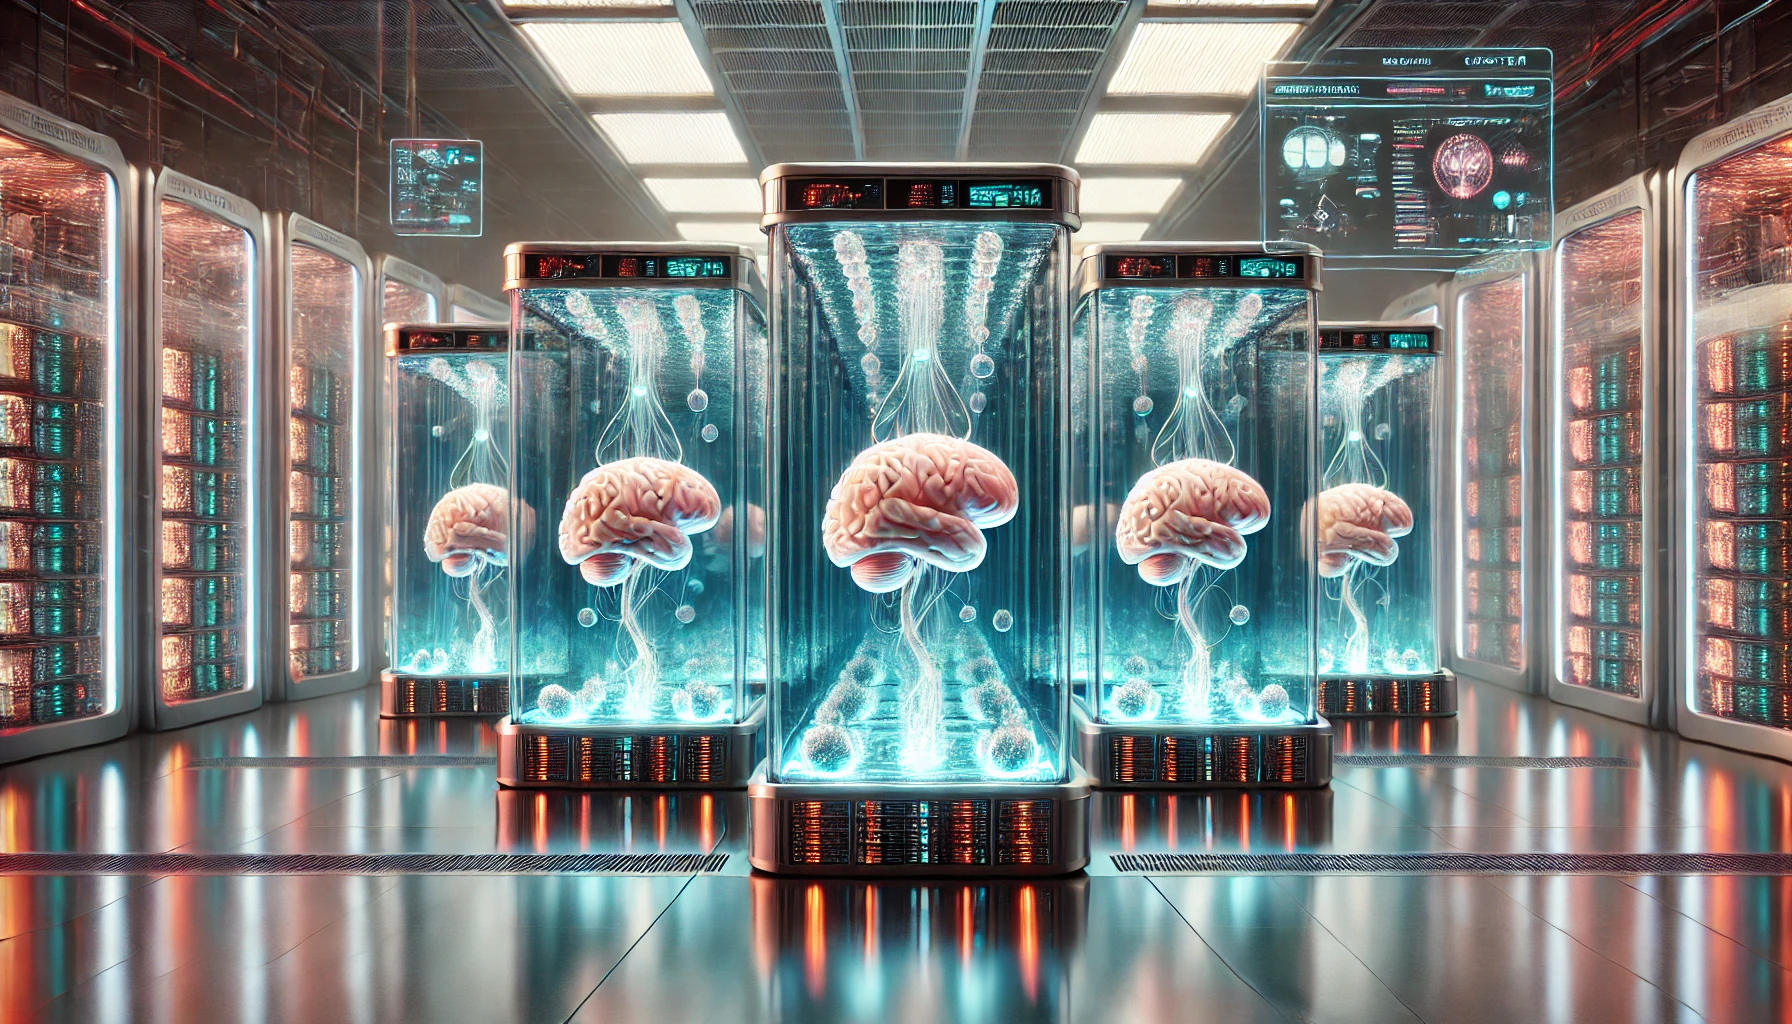
\includegraphics[width=0.8\textwidth]{organoids.png}

    \caption{A dystopic portrayal of a brain organoid data center.}
\end{figure}

The integration of biological and computational principles requires careful attention to how physical systems achieve information processing. Studies of bioelectric signaling reveal sophisticated mechanisms for controlling growth and form in biological tissues \cite{Levin2018}. These bioelectric codes demonstrate how living systems implement computation through direct physical processes rather than abstract symbol manipulation.

Advanced simulation tools enable systematic investigation of physiological signaling in biological tissues \cite{Pietak2017}. These platforms help researchers understand how coherent patterns emerge from complex cellular interactions, providing crucial insights into consciousness-supporting mechanisms. The ability to model and manipulate bioelectric fields offers new approaches for studying how conscious-like processing might emerge in engineered biological systems.

Recent developments in neuromorphic computing have demonstrated remarkable capabilities in artificial neural systems \cite{Merolla2014}. However, these digital implementations fundamentally differ from biological computation in their physical implementation. Understanding these differences helps clarify why consciousness may require specific forms of biological organization rather than merely sophisticated information processing.

The integration of living neural networks with artificial systems presents unique opportunities for investigating consciousness-supporting mechanisms \cite{DeMarse2005}. These hybrid approaches enable systematic examination of how biological neural networks achieve and maintain coherent states while processing information. The ability to interface living neurons with artificial systems provides valuable tools for testing ECC's predictions about consciousness-supporting architectures.

Ethical considerations become increasingly relevant as brain organoids achieve greater sophistication. Recent work has raised important questions about consciousness assessment in cerebral organoids \cite{Lavazza2018}. These ethical challenges require careful consideration as researchers develop more complex biological systems capable of supporting consciousness-like processing.

The experimental use of human brain tissue demands rigorous ethical frameworks \cite{Farahany2018}. As organoid systems become more sophisticated, researchers must carefully consider the potential for conscious-like properties to emerge in these tissues. This ethical dimension becomes particularly significant when developing systems specifically designed to test theories of consciousness.

\begin{figure}[h]
    \centering
    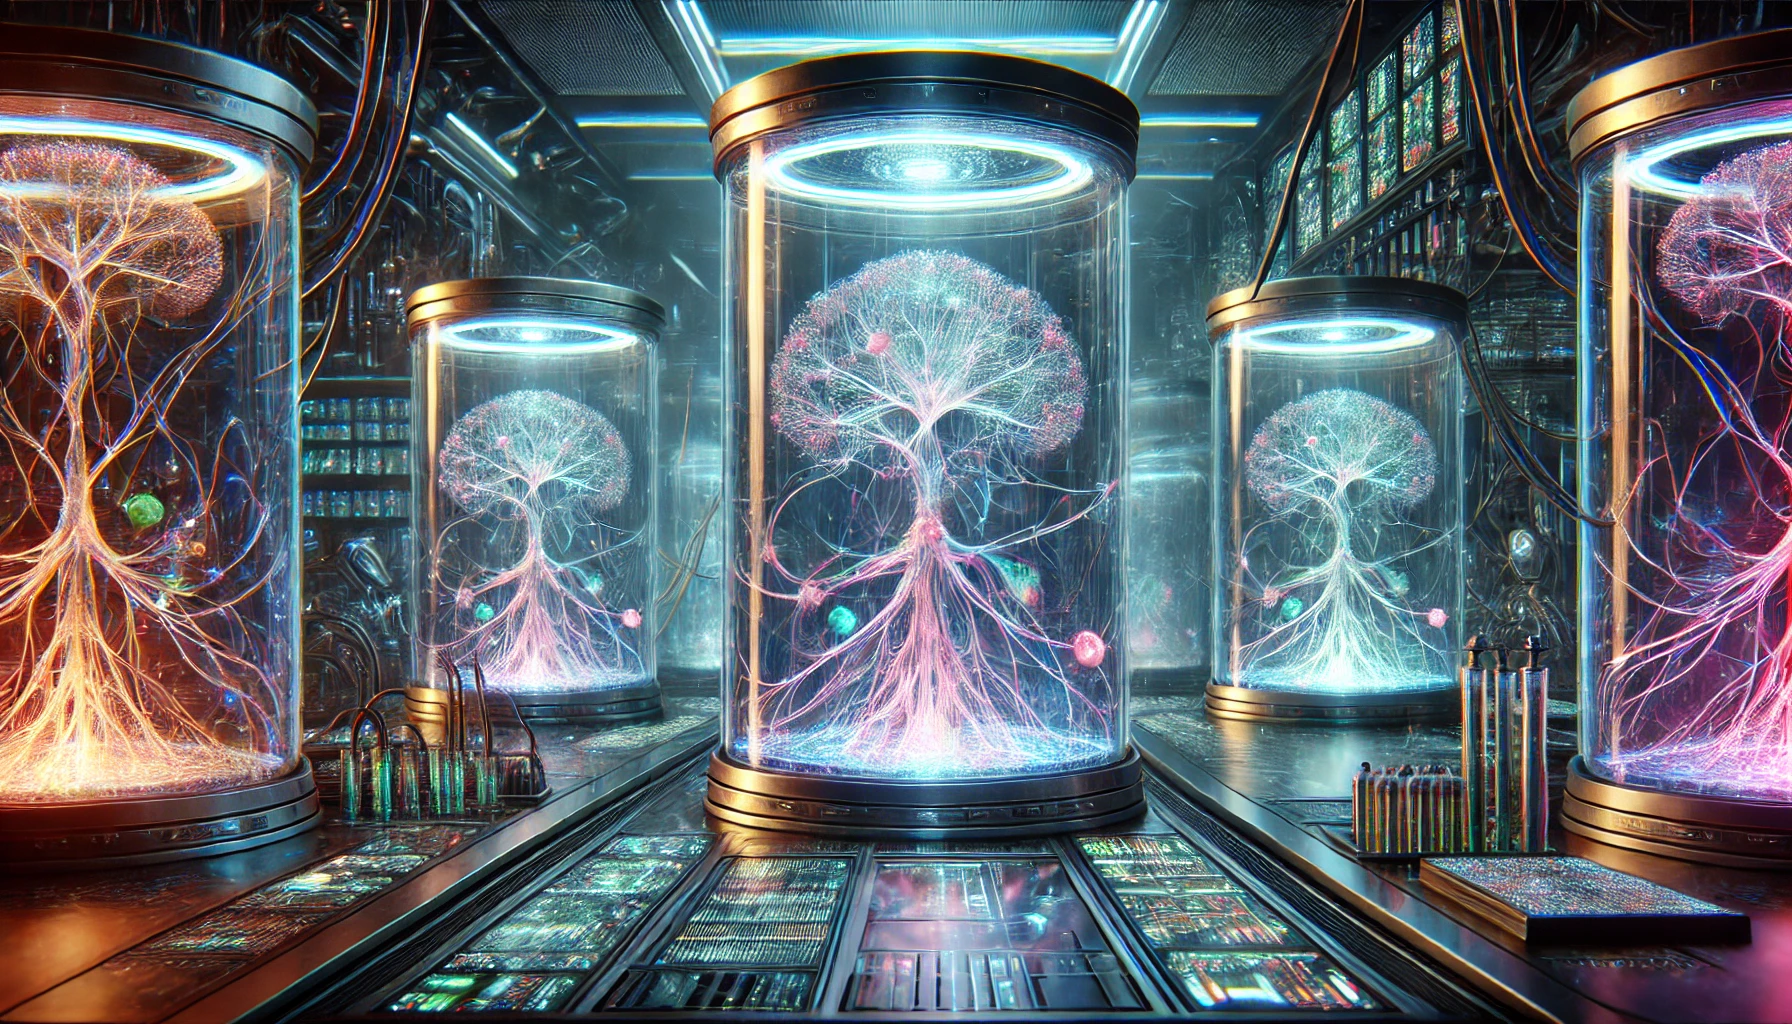
\includegraphics[width=0.8\textwidth]{wetware.png}

    \caption{Wetware computing}
\end{figure}

The integrated systems approach to biological networks reveals fundamental principles about how consciousness-supporting architectures emerge from neural organization \cite{Zhang2016}. By examining how different cellular elements interact to create coherent states, researchers can better understand the physical requirements for conscious processing. This systems-level perspective proves essential for bridging between molecular mechanisms and conscious experience.

Recent work has illuminated how conscious integration depends on physical substrates rather than abstract computation \cite{Krishnan2019}. The specific properties of biological tissues enable forms of information processing that cannot be reduced to traditional computational approaches. Understanding these physical constraints helps explain why consciousness requires particular forms of biological organization.

Advanced organoid and assembloid technologies provide increasingly sophisticated platforms for investigating neural development and function \cite{Saha2020}. These systems enable systematic examination of how neural tissues achieve and maintain coherent states through biological mechanisms. The ability to create more complex neural structures offers new opportunities for studying consciousness-supporting architectures.

The development of bioengineered functional brain-like cortical tissue represents a significant advancement for consciousness research \cite{TangSchomer2014}. These engineered tissues demonstrate how biological systems can achieve sophisticated information processing through direct physical mechanisms rather than abstract computation. Such approaches align with ECC's emphasis on consciousness as emerging from coherent energy dynamics in biological systems.

The future development of brain organoids and wetware computing must carefully balance scientific advancement with ethical considerations. As these systems become more sophisticated, researchers must remain attentive to both the potential for conscious-like properties to emerge and the implications of creating such systems. This careful integration of scientific and ethical considerations will prove essential for advancing our understanding of consciousness while maintaining responsible research practices.

\section{Concrete Empirical Tests}

Below is a non-exhaustive proposal for translating ECC’s theoretical claims into empirically testable studies and operationalized measurements. Because ECC is a broad, multi-scale framework, it necessitates an integrated set of methods drawn from molecular biology, neurophysiology, and systems neuroscience. The underlying principle is to link measurable physical or biological variables, such as energy usage, electromagnetic fields, and astrocyte signals, with conscious states in a manner that ECC specifically predicts and explains.

A useful first step involves defining operational measures of "energetic coherence," beginning at the local level by quantifying electromagnetic activity through local field potentials, EEG/MEG signals, or intracellular voltage measurements; chemical signaling through real-time calcium imaging, microdialysis for neurotransmitters, and metabolic markers such as NADH fluorescence; mechanical processes by assessing tissue pulsations or cytoskeletal tension; and transcriptomic changes through single-cell RNA-seq snapshots in relevant brain regions. At the global scale, researchers can employ multi-electrode arrays or high-density EEG to determine spatiotemporal correlations (coherence or phase-locking) across multiple cortical or subcortical areas. Where feasible, they can also track local metabolic rates using techniques such as fMRI or BOLD signals, with the ultimate aim of extracting a spatially integrated coherence metric.

ECC posits that surpassing a particular threshold of energetic alignment is necessary for consciousness to emerge. A practical strategy for testing this hypothesis is to establish an operational coherence index, potentially computed from amplitude and phase synchrony across different frequencies and brain regions, and then observe whether it correlates with transitions between conscious and unconscious states, such as those induced by anesthesia.

In formulating testable hypotheses, investigators should articulate clear, falsifiable propositions. One central idea is that measurable changes in a proposed energetic coherence index will coincide with the transition from unconsciousness to consciousness, for instance, during the induction and emergence phases of anesthesia. Another hypothesis focuses on the involvement of astrocytic networks, positing that selectively perturbing astrocyte function should reduce local coherence and disrupt conscious experience more profoundly than analogous interventions targeting neurons alone. A related proposition addresses the role of transcriptomic alphabets, predicting systematic shifts in gene expression profiles when specific brain regions become stably integrated into a global conscious state. Further hypotheses explore how artificially modulating local energy flow, through micro-injections of metabolic substrates or inhibitors, should alter coherence in a manner that correlates with disruptions or enhancements of conscious processing.

Various experimental paradigms can be employed to examine these hypotheses. In human studies, noninvasive methods such as EEG or MEG can be combined with advanced source-localization techniques, and the results might be further correlated with FD-NIRS or metabolic imaging where available. Researchers can test whether measured coherence indices align with stages of wakefulness, REM sleep, and deep sleep, or whether a more coherent stress-energy environment leads to more globally integrated responses to TMS-induced perturbations. In animal or invasive studies, multi-electrode arrays in rodent or primate models enable real-time measurement of local coherence, including simultaneous neuronal and astrocytic imaging, while optogenetic or pharmacological manipulations of specific cell populations reveal how local energetic coherence changes. Targeted measures of gene expression across different states (awake, anesthetized, or during distinct behaviors) can also elucidate whether region-specific transcriptomic shifts accompany changes in consciousness. In vitro models such as cortical organoids or brain slices permit tightly controlled manipulations of metabolic substrates, offering insights into how coherence-based bursting patterns might arise or degrade under experimental conditions that mimic or obstruct proposed coherence states.

Operationalizing the sheaf-theoretic and triangulation concepts in ECC can be done by defining local electrode arrays or imaging fields whose overlapping regions are evaluated for similarity or correlated activity. Researchers can then measure whether coherence between non-adjacent areas remains stable across multiple mediating pathways or chains of regions. Recursively applying perturbations and measurements over repeated cycles tests whether local states converge to a stable global coherence pattern or exhibit oscillations and fragmentation instead.

Further refinement involves shifting from the theoretical stress-energy tensor to metrics that can be estimated experimentally, such as an energy flow matrix or flux map derived from electromagnetic, chemical, and mechanical data. Realistic approaches might consider whether local changes in energy distribution appear as redirection flows rather than unaccounted generation or annihilation. Whenever feasible, correlating chemical transmitter release with local electromagnetic changes provides a quantitative window into coupling constants that ECC predicts should be significant.

Evaluating predictions against empirical data involves correlating coherence indices with behavioral measures of consciousness, determining causality by testing whether interventions that alter local or global coherence produce commensurate changes in conscious experience, and fitting simplified computational models with ECC’s rules to known patterns of neural activity. While biological experiments inevitably face practical challenges—such as the complexity of multi-modal data, partial observability of neural processes, and intrinsic noise—an incremental approach allows investigators to test segments of ECC’s framework rather than attempting a single, all-encompassing study.

Despite these challenges, the potential benefits of validating or refining ECC’s main propositions are substantial. A successful series of studies would offer a novel, physically grounded perspective on the unification of conscious experience, providing insights that go beyond conventional computational or information-based accounts of consciousness. By systematically investigating and manipulating energetic coherence in living systems, researchers could either substantiate key aspects of ECC—such as the integral roles of glial coherence, critical energetic thresholds, and path-independent triangulation—or adapt and refine the framework in response to empirical findings.

These considerations naturally lead us to examine novel predictions generated by ECC that could be tested across multiple experimental platforms. The systematic investigation of these predictions requires careful attention to both methodological rigor and ethical implications while maintaining clear connection to empirically measurable phenomena.

\section{Novel Predictions}

The Energetically Coherent Computation framework generates several testable predictions that differentiate it from other theories of consciousness. These predictions span multiple domains of investigation while maintaining clear empirical grounding. Recent theoretical work has emphasized the importance of developing precise, testable hypotheses about conscious processing \cite{Dehaene2014}.

At the biological level, ECC makes specific predictions about neural correlates of consciousness that differ from traditional approaches \cite{Koch2016}. The framework suggests that distinct transcriptomic profiles should correlate with different types of conscious processing, with consciousness-supporting regions demonstrating measurably higher energetic efficiency than those handling unconscious computation.

Large-scale brain networks should demonstrate specific patterns during conscious processing that reflect coherent energy states \cite{Mashour2018}. The framework predicts that transitions between conscious states follow predictable trajectories in terms of energy dynamics, with measurable differences in coherence patterns distinguishing conscious from unconscious neural activity.

Single-nucleus RNA sequencing technologies enable precise testing of ECC's predictions about molecular organization in consciousness-supporting regions \cite{Lake2016}. The framework suggests that regions capable of supporting conscious processing should demonstrate specific patterns of gene expression related to energy management and cellular coherence. These molecular signatures should differ systematically from regions handling unconscious processing.

Transcriptomic diversity across neural populations provides another crucial domain for testing ECC's predictions \cite{Tasic2018}. The framework suggests that consciousness-supporting regions require richer molecular alphabets than those processing information unconsciously. This diversity should correlate specifically with the capacity for maintaining coherent energy states rather than merely reflecting general computational demands.

The developmental trajectory of conscious processing offers particularly promising opportunities for testing ECC's predictions \cite{DehaeneLambertz2015}. The framework suggests that conscious awareness emerges alongside specific patterns of coherence development, with transcriptomic profiles showing characteristic changes that parallel the emergence of conscious capabilities.

These predictions naturally lead to specific experimental protocols for validation across multiple platforms, from cellular systems to intact brains. The systematic investigation of these predictions requires careful attention to both methodological rigor and practical feasibility while maintaining clear connection to established scientific frameworks.

The empirical validation of ECC's predictions requires sophisticated methodologies for measuring and manipulating conscious states. Information integration approaches have demonstrated success in quantifying consciousness-independent neural dynamics \cite{Casali2013}. ECC extends these methods by predicting specific relationships between energy coherence patterns and conscious processing that can be experimentally verified.

Neuroimaging techniques offer powerful tools for detecting consciousness in clinical contexts \cite{Owen2013}. ECC makes specific predictions about how patterns of energetic coherence should correlate with different levels of consciousness, suggesting new approaches for assessing awareness in patients with disorders of consciousness.

The systematic study of consciousness disorders provides crucial opportunities for testing ECC's framework \cite{Giacino2014}. Different disorders should correlate with specific patterns of coherence disruption, while recovery of consciousness should follow predictable trajectories in terms of coherence restoration. These clinical observations can help validate ECC's fundamental predictions about consciousness-supporting mechanisms.

Global workspace dynamics in cortical networks suggest specific mechanisms for conscious processing \cite{Baars2013}. ECC builds on these insights by predicting how energetic coherence patterns support information integration and broadcast across neural networks. These predictions can be tested through careful measurement of energy dynamics during conscious processing.

The investigation of consciousness presents significant methodological challenges \cite{Seth2010}. ECC addresses these challenges by providing concrete, testable predictions about the relationship between physical mechanisms and conscious experience. The framework suggests specific experimental approaches for bridging between subjective experience and objective measurements.

Recent developments in consciousness research have emphasized the importance of no-report paradigms for identifying true neural correlates of consciousness \cite{Tsuchiya2015}. ECC extends these approaches by predicting specific patterns of energetic coherence that should correlate with conscious processing independent of behavioral report.

The integration of information theory with consciousness research offers important tools for testing ECC's predictions \cite{Tononi2016}. However, ECC suggests that information integration alone cannot fully account for conscious experience - specific patterns of energetic coherence must be maintained through biological mechanisms. This distinction generates testable predictions about the physical requirements for consciousness.

Practical measures of information integration in time-series data provide valuable methods for testing consciousness theories \cite{Barrett2011}. ECC builds on these approaches by predicting specific relationships between patterns of energetic coherence and conscious processing. These predictions can be validated through careful measurement of energy dynamics across multiple temporal and spatial scales.

Recent theoretical work has suggested potential convergence between different theories of consciousness \cite{Northoff2020}. ECC contributes to this synthesis by providing concrete predictions about how physical mechanisms support conscious processing. The framework suggests specific experiments that could help resolve apparent contradictions between competing theories.

The development of artificial systems provides another crucial domain for testing ECC's predictions. Unlike traditional computational approaches, ECC suggests that conscious-like processing requires specific forms of physical organization that support coherent energy dynamics. This generates testable predictions about the minimum physical requirements for creating artificial conscious-like systems.

Clinical applications offer particularly promising directions for validating ECC's framework. The theory predicts that different disorders of consciousness should correlate with specific patterns of coherence disruption, while recovery should follow predictable trajectories in terms of energy dynamics. These predictions can be systematically tested through careful clinical observation and measurement.

\newpage
\section{References}
\printbibliography[title={},heading=subbibliography]
%\printbibliography[title={References: Future Directions}]
\end{refsection}